%
% Chapter: Appendix - POSITIVE PARITY INFO
% Modified: 2/16/2015
% Author: James Till Matta
%
%%%%%%%%%%%%%%%%%%%%%%%%%%%%%%%%%%%%%%%%%%%%%%%%%%%%%%%%%%

\chapter{POSITIVE PARITY TRANSITION INFORMATION}
\label{app:pos-par-info}
This appendix contains the full level scheme of \pr{} in Fig. \ref{fig:pp-full-lvl-scheme}. A table of information for the levels in Fig. \ref{fig:pp-full-lvl-scheme} is present in Table \ref{tbl:pp-level-info}. A table of transition information for the transitions in Fig. \ref{fig:pp-full-lvl-scheme} is present in Table \ref{tbl:pp-transition-info}. TODO: Currently both the figure and the table are stand ins with negative parity information.

\begin{landscape}
\begin{figure}[h!]
\centerline{\includegraphics[height=\textheight]{./img/app_pp/135Pr_Np_for_diss.eps}}
	\caption{TODO:GET ACTUAL FULL LEVEL SCHEME. Full level scheme developed for \pr{}.\label{fig:pp-full-lvl-scheme}}
\end{figure}
\end{landscape}

\begin{center}
  \begin{longtable}{|c|c|c|}
    \caption{TABLE OF LEVEL INFORMATION FOR \pr{}, SORTED BY BAND\label{tbl:pp-level-info}\/}\\
        \toprule
 Level Energy &$ J^{\pi} $& Band \\
        \midrule
\endfirsthead % Everything above goes at the top of the 1st page only
% As with the first header, we don't want obscene amounts of space for
% subsequent headings either, and eliminate an em of whitespace.
  \caption[]{{\em Continued}}\\ %The [] argument prevents a duplicate table entries
  \midrule
 Level Energy &$ J^{\pi} $& Band \\
  \midrule
\endhead 
\bottomrule
\endfoot 
  \bottomrule
\endlastfoot % The very last bottom of the table
 358.0 &$ 11/2^{-} $& Yrast \\
 730.7882 &$ 15/2^{-} $& Yrast \\
 1390.9882 &$ 19/2^{-} $& Yrast \\
 2245.1882 &$ 23/2^{-} $& Yrast \\
 3245.2881 &$ 27/2^{-} $& Yrast \\
 4320.7881 &$ 31/2^{-} $& Yrast \\
 5164.7427 &$ 35/2^{-} $& Yrast \\
 5998.6118 &$ 39/2^{-} $& Yrast \\
 6880.2720 &$ 43/2^{-} $& Yrast \\
 7803.1719 &$ 47/2^{-} $& Yrast \\
 8760.1719 &$ 51/2^{-} $& Yrast \\
 1477.80 &$ 17/2^{-} $& $n_w=1$ \\
 2203.80 &$ 21/2^{-} $& $n_w=1$ \\
 2999.80 &$ 25/2^{-} $& $n_w=1$ \\
 3955.4436 &$ 29/2^{-} $& $n_w=1$ \\
 5067.4434 &$ 33/2^{-} $& $n_w=1$ \\
 5113.1436 &$ 33/2^{-} $& Dipole Band 1 \\
 5710.9707 &$ 37/2^{-} $& Dipole Band 1 \\
 6524.3706 &$ 41/2^{-} $& Dipole Band 1 \\
 7502.9321 &$ 45/2^{-} $& Dipole Band 1 \\
 8595.3604 &$ 49/2^{-} $& Dipole Band 1 \\
 5376.4097 &$ 35/2^{-} $& Dipole Band 1 \\
 6095.2910 &$ 39/2^{-} $& Dipole Band 1 \\
 6983.6006 &$ 43/2^{-} $& Dipole Band 1 \\
 8033.0845 &$ 47/2^{-} $& Dipole Band 1 \\
 951.90 &$ 13/2^{-} $& Signature Partner \\
 1433.50 &$ 17/2^{-} $& Signature Partner \\
 2158.50 &$ 21/2^{-} $& Signature Partner \\
 3003.50 &$ 25/2^{-} $& Signature Partner \\
 1927.9199 &$ 19/2^{-} $& Possible $n_w=2$ \\
 2754.3105 &$ (23/2^{-}) $& Possible $n_w=2$ \\
 3517.4814 &$ (27/2^{-}) $& Possible $n_w=2$ \\
 3864.1313 &$ (29/2^{-}) $& Dipole Band 2 \\
 4705.1138 &$ (33/2^{-}) $& Dipole Band 2 \\
 5454.1406 &$ (37/2^{-}) $& Dipole Band 2 \\
 6507.7715 &$ (41/2^{-}) $& Dipole Band 2 \\
 2617.1313 &$ (23/2^{-}) $& Dipole Band 2 \\
 3489.1313 &$ (27/2^{-}) $& Dipole Band 2 \\
 4293.9619 &$ (31/2^{-}) $& Dipole Band 2 \\
 5030.0571 &$ (35/2^{-}) $& Dipole Band 2 \\
 5952.9380 &$ (39/2^{-}) $& Dipole Band 2 \\
 2715.4192 &$ (21/2^{-}) $& Unassigned \\
 3381.9314 &$ (25/2^{-}) $& Unassigned \\
 3531.1313 &$ (27/2^{-}) $& Unassigned \\
\hline \hline
\end{longtable}
\end{center}


\begin{landscape}
\begin{center}
  \begin{longtable}{|c|ccc|ccc|c|c|c|}
    \caption{TABLE OF GAMMA-RAY TRANSITION INFORMATION FOR \pr{} SORTED BY GAMMA-RAY ENERGY\label{tbl:pp-transition-info}\/}\\
        \toprule
$E_i$ &$ Band_i $&$ \rightarrow $&$ Band_f $&$ J^{\pi}_i $&$ \rightarrow $&$ J^{\pi}_f $&$ E_{\gamma} $&$ I_{\gamma} $& Mult. \\
        \midrule
\endfirsthead % Everything above goes at the top of the 1st page only
% As with the first header, we don't want obscene amounts of space for
% subsequent headings either, and eliminate an em of whitespace.
  \caption[]{{\em Continued}}\\ %The [] argument prevents a duplicate table entries
  \midrule
$E_i$ &$ Band_i $&$ \rightarrow $&$ Band_f $&$ J^{\pi}_i $&$ \rightarrow $&$ J^{\pi}_f $&$ E_{\gamma} $&$ I_{\gamma} $& Mult. \\
  \midrule
\endhead 
\bottomrule
\endfoot 
  \bottomrule
\endlastfoot % The very last bottom of the table
%here starts the data
 1478 &$n_w=1$&$ \rightarrow $&Yrast&$ 17/2^{-} $&$ \rightarrow $&$ 19/2^{-} $& 86.8(10) & 0.3(4) & M1 \\
 3531 &Unassigned&$ \rightarrow $&Unassigned&$ (27/2^{-}) $&$ \rightarrow $&$ (25/2^{-}) $& 149.2(10) & 0.29(4) & M1 \\
 952 &Signature Partner&$ \rightarrow $&Yrast&$ 13/2^{-} $&$ \rightarrow $&$ 15/2^{-} $& 221.1(10) & 1.07(16) & M1 \\
 2158 &Signature Partner&$ \rightarrow $&Possible $n_w=2$&$ 21/2^{-} $&$ \rightarrow $&$ 19/2^{-} $& 230.6(10) & 3.3(4) & M1 \\
 5376 &Dipole Band 1&$ \rightarrow $&Dipole Band 1&$ 35/2^{-} $&$ \rightarrow $&$ 33/2^{-} $& 263.3(10) & 0.670(16) & M1 \\
 5376 &Dipole Band 1&$ \rightarrow $&$n_w=1$&$ 35/2^{-} $&$ \rightarrow $&$ 33/2^{-} $& 309.0(10) & 0.690(14) & M1 \\
 5030 &Dipole Band 2&$ \rightarrow $&Dipole Band 2&$ (35/2^{-}) $&$ \rightarrow $&$ (33/2^{-}) $& 324.9(10) & 1.30(17) & M1 \\
 3864 &Dipole Band 2&$ \rightarrow $&Unassigned&$ (29/2^{-}) $&$ \rightarrow $&$ (27/2^{-}) $& 333.0(10) & 1.70(15) & M1 \\
 5711 &Dipole Band 1&$ \rightarrow $&Dipole Band 1&$ 37/2^{-} $&$ \rightarrow $&$ 35/2^{-} $& 334.6(10) & 1.030(20) & M1 \\
 3864 &Dipole Band 2&$ \rightarrow $&Possible $n_w=2$&$ (29/2^{-}) $&$ \rightarrow $&$ (27/2^{-}) $& 346.6(10) & 1.07(5) & M1 \\
 731 &Yrast&$ \rightarrow $&Yrast&$ 15/2^{-} $&$ \rightarrow $&$ 11/2^{-} $& 372.8(10) & 100.0(4) & E2 \\
 3864 &Dipole Band 2&$ \rightarrow $&Dipole Band 2&$ (29/2^{-}) $&$ \rightarrow $&$ (27/2^{-}) $& 375.0(10) & 0.71(3) & M1 \\
 3000 &$n_w=1$&$ \rightarrow $&Dipole Band 2&$ 25/2^{-} $&$ \rightarrow $&$ (23/2^{-}) $& 382.7(10) & 1.11(10) & M1 \\
 6095 &Dipole Band 1&$ \rightarrow $&Dipole Band 1&$ 39/2^{-} $&$ \rightarrow $&$ 37/2^{-} $& 384.3(10) & 0.596(10) & M1 \\
 4705 &Dipole Band 2&$ \rightarrow $&Yrast&$ (33/2^{-}) $&$ \rightarrow $&$ 31/2^{-} $& 384.3(10) & 2.04(7) & M1 \\
 4705 &Dipole Band 2&$ \rightarrow $&Dipole Band 2&$ (33/2^{-}) $&$ \rightarrow $&$ (31/2^{-}) $& 411.2(10) & 1.47(20) & M1 \\
 2617 &Dipole Band 2&$ \rightarrow $&$n_w=1$&$ (23/2^{-}) $&$ \rightarrow $&$ 21/2^{-} $& 413.3(10) & 1.06(10) & M1 \\
 5454 &Dipole Band 2&$ \rightarrow $&Dipole Band 2&$ (37/2^{-}) $&$ \rightarrow $&$ (35/2^{-}) $& 424.1(10) & 0.90(9) & M1 \\
 6524 &Dipole Band 1&$ \rightarrow $&Dipole Band 1&$ 41/2^{-} $&$ \rightarrow $&$ 39/2^{-} $& 429.1(10) & 0.291(4) & M1 \\
 4294 &Dipole Band 2&$ \rightarrow $&Dipole Band 2&$ (31/2^{-}) $&$ \rightarrow $&$ (29/2^{-}) $& 429.8(10) & 2.42(22) & M1 \\
 1928 &Possible $n_w=2$&$ \rightarrow $&$n_w=1$&$ 19/2^{-} $&$ \rightarrow $&$ 17/2^{-} $& 450.1(10) & 3.25(7) & M1 \\
 4321 &Yrast&$ \rightarrow $&Dipole Band 2&$ 31/2^{-} $&$ \rightarrow $&$ (29/2^{-}) $& 456.7(10) & 0.48(7) & M1 \\
 6984 &Dipole Band 1&$ \rightarrow $&Dipole Band 1&$ 43/2^{-} $&$ \rightarrow $&$ 41/2^{-} $& 459.2(10) & 0.188(3) & M1 \\
 2715 &Unassigned&$ \rightarrow $&Yrast&$ (21/2^{-}) $&$ \rightarrow $&$ 23/2^{-} $& 470.2(10) & 1.15(4) & M1 \\
 1434 &Signature Partner&$ \rightarrow $&Signature Partner&$ 17/2^{-} $&$ \rightarrow $&$ 13/2^{-} $& 481.6(10) & 6.9(3) & E2 \\
 1928 &Possible $n_w=2$&$ \rightarrow $&Signature Partner&$ 19/2^{-} $&$ \rightarrow $&$ 17/2^{-} $& 494.4(10) & 0.3(4) & M1 \\
 5953 &Dipole Band 2&$ \rightarrow $&Dipole Band 2&$ (39/2^{-}) $&$ \rightarrow $&$ (37/2^{-}) $& 498.8(10) & 0.81(8) & M1 \\
 3517 &Possible $n_w=2$&$ \rightarrow $&$n_w=1$&$ (27/2^{-}) $&$ \rightarrow $&$ 25/2^{-} $& 517.7(10) & 1.35(7) & M1 \\
 7503 &Dipole Band 1&$ \rightarrow $&Dipole Band 1&$ 45/2^{-} $&$ \rightarrow $&$ 43/2^{-} $& 519.3(10) & 0.1443(24) & M1 \\
 1478 &$n_w=1$&$ \rightarrow $&Signature Partner&$ 17/2^{-} $&$ \rightarrow $&$ 13/2^{-} $& 525.9(10) & 1.50(12) & E2 \\
 8033 &Dipole Band 1&$ \rightarrow $&Dipole Band 1&$ 47/2^{-} $&$ \rightarrow $&$ 45/2^{-} $& 530.2(10) & 0.0647(16) & M1 \\
 2754 &Possible $n_w=2$&$ \rightarrow $&$n_w=1$&$ (23/2^{-}) $&$ \rightarrow $&$ 21/2^{-} $& 550.5(10) & 1.91(6) & M1 \\
 6508 &Dipole Band 2&$ \rightarrow $&Dipole Band 2&$ (41/2^{-}) $&$ \rightarrow $&$ (39/2^{-}) $& 554.8(10) & 0.67(7) & M1 \\
 8595 &Dipole Band 1&$ \rightarrow $&Dipole Band 1&$ 49/2^{-} $&$ \rightarrow $&$ 47/2^{-} $& 562.3(10) & 0.02(3) & M1 \\
 952 &Signature Partner&$ \rightarrow $&Yrast&$ 13/2^{-} $&$ \rightarrow $&$ 11/2^{-} $& 593.9(10) & 9.30(4) & M1 \\
 2754 &Possible $n_w=2$&$ \rightarrow $&Signature Partner&$ (23/2^{-}) $&$ \rightarrow $&$ 21/2^{-} $& 595.8(10) & 1.28(7) & M1 \\
 5711 &Dipole Band 1&$ \rightarrow $&Dipole Band 1&$ 37/2^{-} $&$ \rightarrow $&$ 33/2^{-} $& 597.8(10) & 0.10(12) & E2 \\
 1391 &Yrast&$ \rightarrow $&Yrast&$ 19/2^{-} $&$ \rightarrow $&$ 15/2^{-} $& 660.2(10) & 77.71(3) & E2 \\
 3382 &Unassigned&$ \rightarrow $&Unassigned&$ (25/2^{-}) $&$ \rightarrow $&$ (21/2^{-}) $& 666.5(10) & 0.6(2) & E2 \\
 2617 &Dipole Band 2&$ \rightarrow $&Possible $n_w=2$&$ (23/2^{-}) $&$ \rightarrow $&$ 19/2^{-} $& 689.2(10) & 6.18(13) & E2 \\
 1434 &Signature Partner&$ \rightarrow $&Yrast&$ 17/2^{-} $&$ \rightarrow $&$ 15/2^{-} $& 702.7(10) & 1.8(5) & M1 \\
 3955 &$n_w=1$&$ \rightarrow $&Yrast&$ 29/2^{-} $&$ \rightarrow $&$ 27/2^{-} $& 710.2(10) & 0.320(18) & M1 \\
 6095 &Dipole Band 1&$ \rightarrow $&Dipole Band 1&$ 39/2^{-} $&$ \rightarrow $&$ 35/2^{-} $& 718.9(10) & 0.074(4) & E2 \\
 2158 &Signature Partner&$ \rightarrow $&Signature Partner&$ 21/2^{-} $&$ \rightarrow $&$ 17/2^{-} $& 725.0(10) & 3.9(4) & E2 \\
 2204 &$n_w=1$&$ \rightarrow $&$n_w=1$&$ 21/2^{-} $&$ \rightarrow $&$ 17/2^{-} $& 726.0(10) & 6.28(5) & E2 \\
 3489 &Dipole Band 2&$ \rightarrow $&Possible $n_w=2$&$ (27/2^{-}) $&$ \rightarrow $&$ (23/2^{-}) $& 734.8(10) & 0.161(20) & E2 \\
 5030 &Dipole Band 2&$ \rightarrow $&Dipole Band 2&$ (35/2^{-}) $&$ \rightarrow $&$ (31/2^{-}) $& 736.1(10) & 0.03(4) & E2 \\
 1478 &$n_w=1$&$ \rightarrow $&Yrast&$ 17/2^{-} $&$ \rightarrow $&$ 15/2^{-} $& 747.0(10) & 12.00(7) & M1 \\
 5454 &Dipole Band 2&$ \rightarrow $&Dipole Band 2&$ (37/2^{-}) $&$ \rightarrow $&$ (33/2^{-}) $& 749.0(10) & 0.03(4) & E2 \\
 3000 &$n_w=1$&$ \rightarrow $&Yrast&$ 25/2^{-} $&$ \rightarrow $&$ 23/2^{-} $& 754.6(10) & 1.92(3) & M1 \\
 3517 &Possible $n_w=2$&$ \rightarrow $&Possible $n_w=2$&$ (27/2^{-}) $&$ \rightarrow $&$ (23/2^{-}) $& 763.2(10) & 1.24(13) & E2 \\
 2158 &Signature Partner&$ \rightarrow $&Yrast&$ 21/2^{-} $&$ \rightarrow $&$ 19/2^{-} $& 767.5(10) & 0.7(6) & M1 \\
 2204 &$n_w=1$&$ \rightarrow $&Signature Partner&$ 21/2^{-} $&$ \rightarrow $&$ 17/2^{-} $& 770.3(10) & 0.0(4) & E2 \\
 3531 &Unassigned&$ \rightarrow $&Possible $n_w=2$&$ (27/2^{-}) $&$ \rightarrow $&$ (23/2^{-}) $& 776.8(10) & 0.96(8) & E2 \\
 3000 &$n_w=1$&$ \rightarrow $&$n_w=1$&$ 25/2^{-} $&$ \rightarrow $&$ 21/2^{-} $& 796.0(10) & 3.50(9) & E2 \\
 4294 &Dipole Band 2&$ \rightarrow $&Dipole Band 2&$ (31/2^{-}) $&$ \rightarrow $&$ (27/2^{-}) $& 804.8(10) & 0.86(8) & E2 \\
 2204 &$n_w=1$&$ \rightarrow $&Yrast&$ 21/2^{-} $&$ \rightarrow $&$ 19/2^{-} $& 812.8(10) & 7.60(15) & M1 \\
 6524 &Dipole Band 1&$ \rightarrow $&Dipole Band 1&$ 41/2^{-} $&$ \rightarrow $&$ 37/2^{-} $& 813.4(10) & 0.03(4) & E2 \\
 2754 &Possible $n_w=2$&$ \rightarrow $&Possible $n_w=2$&$ (23/2^{-}) $&$ \rightarrow $&$ 19/2^{-} $& 826.4(10) & 1.06(6) & E2 \\
 5999 &Yrast&$ \rightarrow $&Yrast&$ 39/2^{-} $&$ \rightarrow $&$ 35/2^{-} $& 833.9(10) & 3.04(7) & E2 \\
 4705 &Dipole Band 2&$ \rightarrow $&Dipole Band 2&$ (33/2^{-}) $&$ \rightarrow $&$ (29/2^{-}) $& 841.0(10) & 0.18(3) & E2 \\
 3000 &$n_w=1$&$ \rightarrow $&Signature Partner&$ 25/2^{-} $&$ \rightarrow $&$ 21/2^{-} $& 841.3(10) & 0.47(11) & E2 \\
 5165 &Yrast&$ \rightarrow $&Yrast&$ 35/2^{-} $&$ \rightarrow $&$ 31/2^{-} $& 844.0(10) & 4.94(10) & E2 \\
 3004 &Signature Partner&$ \rightarrow $&Signature Partner&$ 25/2^{-} $&$ \rightarrow $&$ 21/2^{-} $& 845.0(10) & 1.37(15) & E2 \\
 2245 &Yrast&$ \rightarrow $&Yrast&$ 23/2^{-} $&$ \rightarrow $&$ 19/2^{-} $& 854.2(10) & 35.80(3) & E2 \\
 5165 &Yrast&$ \rightarrow $&Dipole Band 2&$ 35/2^{-} $&$ \rightarrow $&$ (31/2^{-}) $& 870.8(10) & 0.62(6) & E2 \\
 3489 &Dipole Band 2&$ \rightarrow $&Dipole Band 2&$ (27/2^{-}) $&$ \rightarrow $&$ (23/2^{-}) $& 872.0(10) & 2.96(9) & E2 \\
 6880 &Yrast&$ \rightarrow $&Yrast&$ 43/2^{-} $&$ \rightarrow $&$ 39/2^{-} $& 881.7(10) & 2.70(7) & E2 \\
 6984 &Dipole Band 1&$ \rightarrow $&Dipole Band 1&$ 43/2^{-} $&$ \rightarrow $&$ 39/2^{-} $& 888.3(10) & 0.0450(8) & E2 \\
 3517 &Possible $n_w=2$&$ \rightarrow $&Dipole Band 2&$ (27/2^{-}) $&$ \rightarrow $&$ (23/2^{-}) $& 900.4(10) & 0.97(5) & E2 \\
 3531 &Unassigned&$ \rightarrow $&Dipole Band 2&$ (27/2^{-}) $&$ \rightarrow $&$ (23/2^{-}) $& 914.0(10) & 0.53(6) & E2 \\
 7803 &Yrast&$ \rightarrow $&Yrast&$ 47/2^{-} $&$ \rightarrow $&$ 43/2^{-} $& 922.9(10) & 1.77(6) & E2 \\
 3955 &$n_w=1$&$ \rightarrow $&$n_w=1$&$ 29/2^{-} $&$ \rightarrow $&$ 25/2^{-} $& 955.6(10) & 1.51(4) & E2 \\
 8760 &Yrast&$ \rightarrow $&Yrast&$ 51/2^{-} $&$ \rightarrow $&$ 47/2^{-} $& 957.0(10) & 1.39(5) & E2 \\
 7503 &Dipole Band 1&$ \rightarrow $&Dipole Band 1&$ 45/2^{-} $&$ \rightarrow $&$ 41/2^{-} $& 978.6(10) & 0.0156(8) & E2 \\
 3245 &Yrast&$ \rightarrow $&Yrast&$ 27/2^{-} $&$ \rightarrow $&$ 23/2^{-} $& 1000.1(10) & 9.62(19) & E2 \\
 4294 &Dipole Band 2&$ \rightarrow $&Yrast&$ (31/2^{-}) $&$ \rightarrow $&$ 27/2^{-} $& 1048.7(10) & 2.14(9) & E2 \\
 8033 &Dipole Band 1&$ \rightarrow $&Dipole Band 1&$ 47/2^{-} $&$ \rightarrow $&$ 43/2^{-} $& 1049.5(10) & 0.0250(8) & E2 \\
 4321 &Yrast&$ \rightarrow $&Yrast&$ 31/2^{-} $&$ \rightarrow $&$ 27/2^{-} $& 1075.5(10) & 5.72(13) & E2 \\
 8595 &Dipole Band 1&$ \rightarrow $&Dipole Band 1&$ 49/2^{-} $&$ \rightarrow $&$ 45/2^{-} $& 1092.4(10) & 0.007(8) & E2 \\
 5067 &$n_w=1$&$ \rightarrow $&$n_w=1$&$ 33/2^{-} $&$ \rightarrow $&$ 29/2^{-} $& 1112.0(10) & 0.734(20) & E2 \\
 5113 &Dipole Band 1&$ \rightarrow $&$n_w=1$&$ 33/2^{-} $&$ \rightarrow $&$ 29/2^{-} $& 1157.7(10) & 0.59(14) & E2 \\
 1928 &Possible $n_w=2$&$ \rightarrow $&Yrast&$ 19/2^{-} $&$ \rightarrow $&$ 15/2^{-} $& 1197.1(10) & 2.2(3) & E2 \\
 2617 &Dipole Band 2&$ \rightarrow $&Yrast&$ (23/2^{-}) $&$ \rightarrow $&$ 19/2^{-} $& 1226.1(10) & 4.54(6) & E2 \\
 3489 &Dipole Band 2&$ \rightarrow $&Yrast&$ (27/2^{-}) $&$ \rightarrow $&$ 23/2^{-} $& 1243.9(10) & 1.20(8) & E2 \\
 3517 &Possible $n_w=2$&$ \rightarrow $&Yrast&$ (27/2^{-}) $&$ \rightarrow $&$ 23/2^{-} $& 1272.3(10) & 0.69(10) & E2 \\
 3531 &Unassigned&$ \rightarrow $&Yrast&$ (27/2^{-}) $&$ \rightarrow $&$ 23/2^{-} $& 1285.9(10) & 2.07(4) & E2 \\
 2754 &Possible $n_w=2$&$ \rightarrow $&Yrast&$ (23/2^{-}) $&$ \rightarrow $&$ 19/2^{-} $& 1363.3(10) & 1.01(12) & E2 \\
\hline \hline
\end{longtable}
\end{center}
\end{landscape}